\title{LEZIONE 6 07/04/2020}\newline
\textbf{link} \href{https://web.microsoftstream.com/video/47324732-47d3-4965-81ca-e0ed065beb5a}{clicca qui}
\section{Statica del punto materiale}
\subsection{Equazioni caridnali della statica per il punto materiale}
Supponiamo di avere un corpo puntiforme di massa $m$ su cui agiscono diverse forze $F_1, F_2,\dots, F_i$.\newline
\newline
Quello che vogliamo fare è stabilire le condizioni per le quali il sistema è in \textbf{equilibrio}, ovvere per cui il punto materiale non si muove.\newline
\newline
\textbf{Condizione necessaria e sufficiente per avere equilibrio in un punto materiale è che si annullino tutte le forze applicate al punto.}\newline
\newline
Imporre questa condizione significa imporre la seguente equazione:
\[
    \vec{R} = \sum_{i}\vec{F}_i = 0
\] 
dove per $\vec{R}$ si intende la risultante delle forze.\newline
Questa equazione si può proiettare lungo gli assi $X$ e $Y$ e ottenere quindi un sistema scalare che prende il nome di \textbf{equazioni cardinali della statica}:
\[
    \begin{cases}
        R_x = 0\\
        R_y = 0
    \end{cases}
\]

Queste equazioni cardinali della statica ci servono per:
\begin{itemize}
    \item Calcolare le reazioni vincolari;
    \item Note forze, calcolare la posizione di euilibrio statico;
    \item Oppure nota la posizione di equilibrio, calcolare le forze attive.
\end{itemize}
\ \newline
Vediamo come procedere operativamente: si prende il punto materiale, lo si isola, si mettono in evidenza tutte le forze che agiscono su di esso, sia quelle attive, sia quelle reattive. Infine si scrivono le equazioni cardinali della statica.\newline
\newline
\textbf{es.} \newline
[immagine dagli appunti del prof]
\begin{center}
    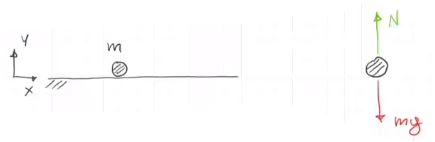
\includegraphics[height=3cm]{../lezione6/img1.JPG}
\end{center}
Un punto materiale $m$ fermo su un piano ci permette di dedurre che esiste una forza vincolare $N$ che contrasta la forza di gravità $mg$.\newline
\newline
Equazioni cardinali della statica:
\[
    \begin{cases}
        R_x = 0\\
        R_y = 0
    \end{cases} \; \rightarrow  \; R_y = N-mg = 0 \; \rightarrow  \; N = mg
\]
\rule{\textwidth}{0,4pt}
\newline
\subsection{Reazioni vincolari}
Le \textbf{reazioni vincolari} sono le forze trasmesse attraverso i vincoli.\newline
\newline
Le reazioni vincolari si comportano in base ai movimenti impediti dal vincolo stesso. Si hanno quindi tante reazioni vincolari quanti sono i gradi di libertà soppressi dal vincolo.
\subsubsection{Incastro}
[immagine dagli appunti del prof]
\begin{center}
    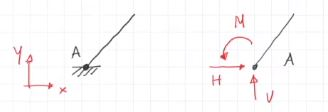
\includegraphics[height=3cm]{../lezione6/img2.JPG}
\end{center}
L'incastro è un vincolo triplo, dunque ha tre reazioni vincolari: $H, V, M$.
\subsubsection{Cerniera}
[immagine dagli appunti del prof]
\begin{center}
    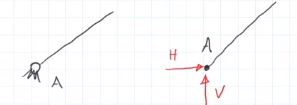
\includegraphics[height=3cm]{../lezione6/img3.JPG}
\end{center}
La cerniera è un vincolo doppio, dunque ha due reazioni vincolari: $H, V$.
\subsubsection{Pattino}
[immagine dagli appunti del prof]
\begin{center}
    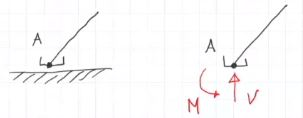
\includegraphics[height=3cm]{../lezione6/img4.JPG}
\end{center}
Il pattino è un vincolo doppio, dunque ha due reazioni vincolari: $M, V$.
\subsubsection{Manicotto}
[immagine dagli appunti del prof]
\begin{center}
    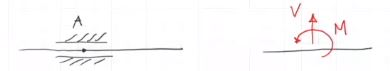
\includegraphics[height=3cm]{../lezione6/img5.JPG}
\end{center}
Il manicotto è un vincolo doppio, dunque ha due reazioni vincolari: $M, V$.
\subsubsection{Carrello-cerniera}
[immagine dagli appunti del prof]
\begin{center}
    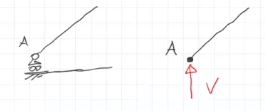
\includegraphics[height=3cm]{../lezione6/img6.JPG}
\end{center}
Il manicotto è un vincolo singolo, dunque ha una sola reazioni vincolari: $V$.
\newline
\newline
\textbf{es.} \newline
[immagine dagli appunti del prof]
\begin{center}
    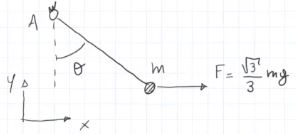
\includegraphics[height=3cm]{../lezione6/img7.JPG}
\end{center}
Un punto con massa $m$ in un piano verticale ha applicata una forza $F$ ed è collagato con una fune inestensibile e incomprimibile (cioè indeformabile e priva di massa) a una cerniera $A$.\newline
\newline
Durante il processo di isolamento del punto di massa $m$ devo tenere in mente la presenza della fune che, siccome è incomprimibile e inestensibile, trasmette la forza della cerniera $A$.\newline
[immagine dagli appunti del prof]
\begin{center}
    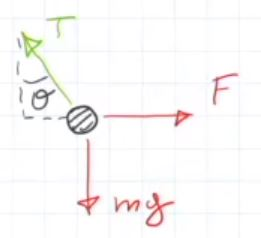
\includegraphics[height=3cm]{../lezione6/img8.JPG}
\end{center}
Scriviamo ora le equazion icardinali della statica lungo l'asse $X$ e lungo l'asse $Y$:
\[
    \begin{cases}
        R_x = 0\\
        R_y=0
    \end{cases} \rightarrow  \begin{cases}
        F-T sin(\theta) = 0\\
        T cos(\theta) - mg = 0
    \end{cases} \rightarrow \begin{cases}
        F = T sin(\theta)\\
        mg = T cos(\theta)
    \end{cases} \rightarrow \begin{cases}
        \frac{\cancel{T} sin(\theta)}{\cancel{T} cos(\theta)} = tan(\theta) = \frac{F}{mg} = \frac{\sqrt{3}}{3} \rightarrow \theta = 30^0\\
        T = \frac{F}{sin(\theta)} = \frac{2}{3}\sqrt{3}mg
    \end{cases}
\]
Possiamo quindi interpretare le forze in gioco, considerando che deve sempre valere il \textbf{principio di azione-reazione}:\newline
[immagine dagli appunti del prof]
\begin{center}
    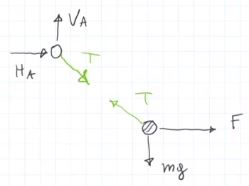
\includegraphics[height=3cm]{../lezione6/img9.JPG}
\end{center}
Dunque ora le forze vincolari sono
\[
    \begin{cases}
        V_A = mg\\
        H_A = -F
    \end{cases}
\]
\rule{\textwidth}{0,4pt}
\newpage
\section{Statica del corpo rigido}
\subsection{equazioni cardinali della statica per il corpo rigido}
L'annullamento della risultante delle forze applicate non è più una condizione sufficiente se si parla di corpi rigidi. Infatti per i corpi rigidi si hanno tre gradi di libertà e questa condizione ci permette di trovare solo due equazioni.\newline
\newline
La nuova \textbf{condizione necessaria e sufficiente per l'equilibrio di un corpo rigido} è che si annulli la risultante di tutte le forze ed il momento rispetto ad un generico polo $O$ di tutte le forze e coppie attive e reattive applicate al corpo stesso.\newline
\newline
Traducendo questa definizione in equazioni otteniamo le \textbf{equazioni cardinali della statica per il corpo rigido}:
\[
    \begin{cases}
        \vec{R} = \sum_{i} \vec{F}_i = 0\\
        \vec{M}_O = \sum_{i} (P_i - O) \land \vec{F}_i + \sum_{j} \vec{C}_j = 0
    \end{cases}
\]
dove $\sum_{i} (P_i - O) \land \vec{F}_i$ rappresenta il \textbf{momento di una forza} e $\sum_{j} \vec{C}_j$ una \textbf{coppia}.\newline
\newline
Da questo sistema otteniamo tre equazioni:
\[
    \begin{cases}
        R_x = 0\\
        R_y = 0\\
        M_O = 0
    \end{cases}
\]
A queste tre equazioni si può sostituire una delle prime due con l'annullamento dei momenti rispetto a un altro polo $Q$:
\[
    \begin{cases}
        R_x = 0\\
        M_O = 0\\
        M_Q = 0
    \end{cases}
\]
a patto che il segmento $OQ$ non sia perpendicolare all'asse delle $X$.\newline
Infine si può ripetere l'ultimo passaggio sostituendo la prima equazione con un altro momento:
\[
    \begin{cases}
        M_O = 0\\
        M_Q = 0\\
        M_P = 0
    \end{cases}
\]
a patto che $O,Q,P$ non siano allineati.\newline
\newline
Le equazioni cardinali della statica mi serviranno per:
\begin{itemize}
    \item calcolare le reazioni vincolari;
    \item definire una posizione di equilibrio, se sono note le forze attive esterne al corpo rigido;
    \item oppure definire le forze attive per mantenere una posizione di equilibrio assegnata. 
\end{itemize}
Notiamo inoltre che questo è possibile solo se il copro è vincolato in maniera isostatica o ipostatica, cioè se il numero di relazioni di vincolo è minore o uguale del numero di gradi di libertà iniziali (che nel caso di corpo singolo sono $3$).
\newline
\newline
Il tipico procedimento analitico è estremamente simile a quello che si fa per il caso del punto materiale:
\begin{itemize}
    \item isolare il corpo rigido;
    \item mettere in evidenza le forze attive e reattive;
    \item applicare le equazioni cardinali della statica.
\end{itemize}
\subsection{Momento di una forza}
[immagine dagli appunti del prof]
\begin{center}
    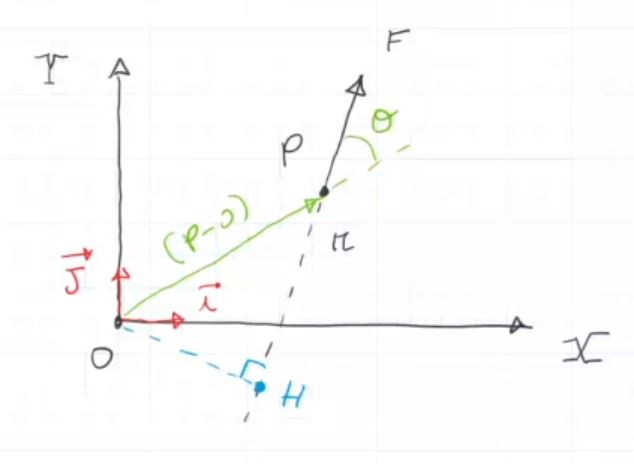
\includegraphics[height=3cm]{../lezione6/img10.JPG}
\end{center}
Data una forza $F$ applicatta a un punto $P$, detto \textbf{punto di applicazione della forza}. Invece $r$ prende il nome di \textbf{retta di applicazione della forza}.\newline
\newline
Il momento rispetto al polo $O$ (in questo caso origine del sistema) per definizione è:
\[
    \vec{M}_O = (P-O) \land \vec{F} = \bar{PO} |\vec{F}| sin(\theta)
\]
Notiamo che $\bar{PO} sin(\theta) = \bar{OH}$, quindi possiamo scrivere:
\[
    \vec{M}_O = |\vec{F}| \cdot  \bar{OH} \vec{k} = \text{forza per braccio}\; 
\]
dove $\bar{OH}$ prende il nome di \textbf{braccio della forza}.\newline
\newline
Notiamo inoltre che se spostassi il punto di applicazione $P$ lungo la retta $r$ di applicazione, il braccio e quindi anche il momento non cambiarebbero.\newline
\newline
Notiamo inoltre il momento è sempre in direzione $\vec{k}$, cioè uscente dal foglio.
\subsection{Coppia}
Una \textbf{coppia} è un sistema di due forze che ha risultante nulla, ma momento diverso da zero.\newline
\newline
[immagine dagli appunti del prof]
\begin{center}
    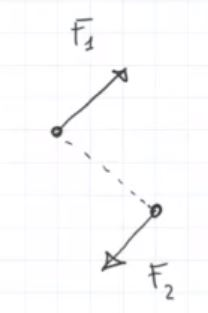
\includegraphics[height=3cm]{../lezione6/img11.JPG}
\end{center}
\ \newline
Perchè questo sia possibile ci devono essere delle condizioni:
\begin{itemize}
    \item $|\vec{F}_1| = |\vec{F}_2| = F$
    \item $\vec{F}_1 \parallel \vec{F}_2$
    \item $\vec{F}_1 = - \vec{F}_2$
\end{itemize}
\ \newline
Se queste condizioni sono rispettate allora siamo in presenza di una coppia, e quindi possiamo sostituire le due forze con una coppia che ha valore pari al modulo delle forze per la distanza $d$ fra i punti di applicazioni:
\[
    \vec{C} = F d \vec{k}
\]
\ \newline
Notiamo che le coppie non dipendono dal polo preso in considerazione.\newline
\newline
\textbf{es.} \newline
[immagine dagli appunti del prof]
\begin{center}
    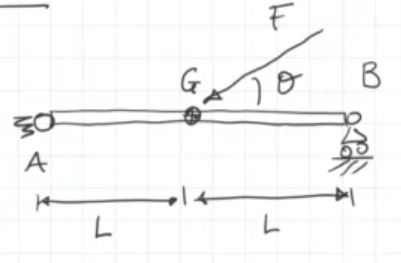
\includegraphics[height=3cm]{../lezione6/img12.JPG}
\end{center}
In questo esempio $n_O = 3 gdl$, $n_v = 2+1 = 3 gdv$ e quindi $n = 0 gdl$. La struttura è isostatica.\newline
\newline
Isoliamo la trave:\newline
[immagine dagli appunti del prof]
\begin{center}
    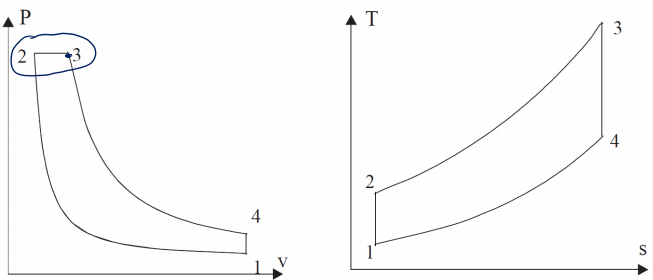
\includegraphics[height=3cm]{../lezione6/img13.jpg}
\end{center}
Abbiamo quindi un sistema in tre incognite $H_A, V_A, V_B$, che possiamo trovare con le equazioni cardinali della statica.
\[
    \begin{cases}
        R_x = 0\\
        R_y = 0\\
        M_A = 0
    \end{cases} \rightarrow \begin{cases}
        H_A - F cos(\theta) = 0\\
        V_A + V_B - F sin(\theta) = 0\\
        - F sin(\theta) L + V_B 2 L = 0
    \end{cases} \rightarrow \begin{cases}
        H_A = F cos(\theta)\\
        V_B = \frac{F}{2} sin(\theta)
        V_A = \frac{F}{2} sin(\theta)
    \end{cases}
\]
con $L$ metà della lunghezza dell'asta.\newline
Capiamo ora la terza delle equazioni cardinali della statica, cioè quella sul momento rispetto al polo $A$. Tutti i vettori forza ($H_A, V_A, F cos(\theta)$), che hanno retta di applicazione passante per il punto $A$ avranno braccio nullo e di conseguenza momento nullo. Gli unici vettori forza con momento non nullo sono quindi $F sin(\theta)$ e $V_B$.\newline
\newline
La scelta del polo è arbitraria, in questo esercizio abbiamo deciso di usare $A$ come polo per pura comodità. \newline
\rule{\textwidth}{0,4pt}
\textbf{es.} \newline
[immagine dagli appunti del prof]
\begin{center}
    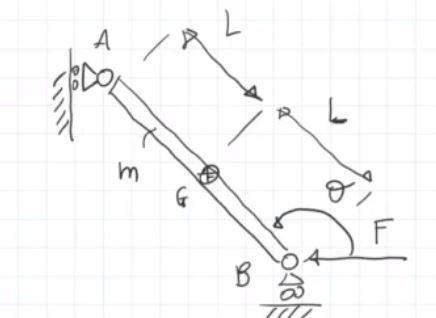
\includegraphics[height=3cm]{../lezione6/img14.JPG}
\end{center}
Assumiamo questo sistema in un piano verticale e di avere $\theta$ noto.\newline
\newline
Calcoliamo i gradi di libertà: $n_O - n_V = n = 3 - 2 = 1 gdl$ che è $\theta$. Il sistema è un meccanismo ipostatico.\newline
\newline
Isoliamo ora la trave e analiziamo le forze:\newline
[immagine dagli appunti del prof]
\begin{center}
    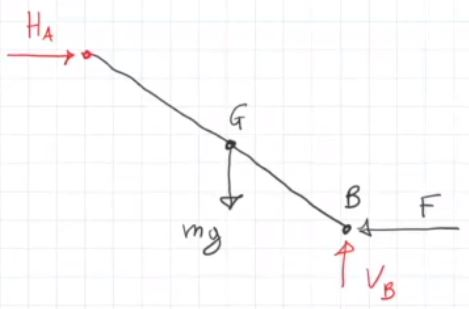
\includegraphics[height=3cm]{../lezione6/img15.JPG}
\end{center}
Impostiamo le equazioni cardinali della statica, considerando come polo dei momenti il punto $C = $ CIR:\newline
[immagine dagli appunti del prof]
\begin{center}
    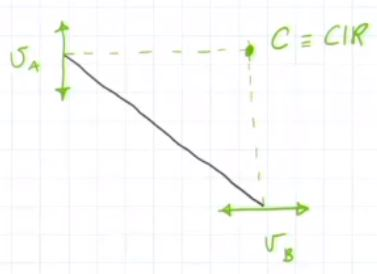
\includegraphics[height=3cm]{../lezione6/img16.JPG}
\end{center} 
[immagine dagli appunti del prof]
\begin{center}
    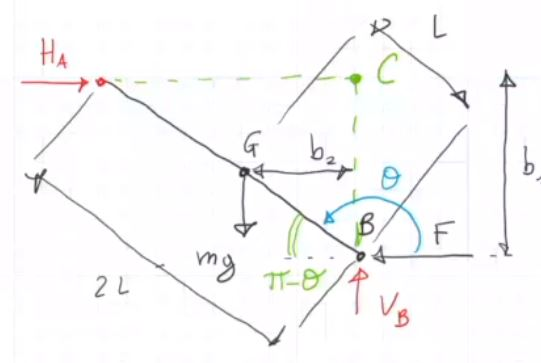
\includegraphics[height=3cm]{../lezione6/img17.JPG}
\end{center} 
\[
    \begin{cases}
        R_x = 0\\
        R_y = 0\\
        M_c = 0
    \end{cases} \rightarrow \begin{cases}
        R_x = 0\\
        R_y = 0\\
        -Fb_1 + mg b_2 = 0
    \end{cases}
\]
Con $b_1 = 2l sin (\pi - \theta) = 2 L sin( \theta)$ e $b_2 = L cos(\pi - \theta) = -L cos(\theta)$.\newline
Nel calcolo del momento per la forza $F$, esso viene posto negativo per convenzione, infatti la forza $F$ fa girare in senso orario l'asta attorno al polo $C$.
\[
    \begin{cases}
        V_B = mg\\
        H_A = F\\
        F = - \frac{mg cos(\theta)}{2 sin(\theta)} = - \frac{mg}{2 tan(\theta)}
    \end{cases}
\]
\rule{\textwidth}{0,4pt}